\section{Task 2: Matrix Games}

Matrix games provide canonical testbeds for studying the interaction between learning algorithms and game-theoretic concepts in multi-agent systems. They are simple, fully specified by payoff matrices, and capture key tradeoffs that appear in more complex environments. In this work, four well-established benchmark games are considered: the \emph{Stag Hunt} (a coordination game), the \emph{Subsidy Game} (a coordination game with asymmetric incentives), \emph{Matching Pennies} (a zero-sum game), and the \emph{Prisoner’s Dilemma} (a social dilemma). Each of these games highlights distinct strategic patterns such as risk-dominance, dominance by defection, or the absence of pure strategy equilibria. The Nash equilibria and Pareto optimal outcomes listed below give insight into the structure of the games. Then agents learn to play these games using various learning algorithms to give insight into how learning agents behave in different strategic settings. Finally the replicator dynamicss of the algorithms are plotted to see if the theoretical predictions match the empirical results.

\begin{figure}[h]
    \centering
    \scalebox{0.85}{ % adjust scaling factor as needed
    \begin{tabular}{c c c c}
    % Stag Hunt
    \begin{tabular}{c|c c}
        & S & H \\
        \hline
        S & (1,1) & (0,2/3) \\
        H & (2/3,0) & (2/3,2/3) \\
    \end{tabular}
    &
    % Subsidy Game
    \begin{tabular}{c|c c}
        & S1 & S2 \\
        \hline
        S1 & (12,12) & (0,11) \\
        S2 & (0,11) & (10,10) \\
    \end{tabular}
    &
    % Matching Pennies
    \begin{tabular}{c|c c}
        & H & T \\
        \hline
        H & (1,-1) & (-1,1) \\
        T & (-1,1) & (1,-1) \\
    \end{tabular}
    &
    % Prisoner's Dilemma
    \begin{tabular}{c|c c}
        & C & D \\
        \hline
        C & (3,3) & (0,5) \\
        D & (5,0) & (1,1) \\
    \end{tabular}
    \end{tabular}
    }
    \caption{Payoff matrices of the four benchmark games: Stag Hunt, Subsidy Game, Matching Pennies, and Prisoner’s Dilemma.}
\end{figure}



\subsection{Nash Equilibria and Pareto Optimal Outcomes}

The four benchmark games are analyzed in terms of their Nash equilibria and Pareto optimal outcomes, based on the payoff matrices defined above.

\paragraph{Stag Hunt.}  
The Stag Hunt is a coordination game. Two pure strategy Nash equilibria exist: $(S,S)$ and $(H,H)$. In addition, there is a mixed equilibrium where each player hunts stag with probability $\tfrac{2}{3}$ and hare with probability $\tfrac{1}{3}$. The unique Pareto optimal outcome is $(S,S)$, which strictly improves upon all other outcomes for both players.

\paragraph{Subsidy Game.}  
The Subsidy Game is also a coordination game. Here, $(S_{1},S_{1})$ is the unique Nash equilibrium, since $S_{1}$ strictly dominates $S_{2}$ for the second player. The only Pareto optimal outcome is likewise $(S_{1},S_{1})$, as it yields the highest joint payoff.

\paragraph{Matching Pennies.}  
Matching Pennies is a constant-sum (zero-sum) game. No pure strategy Nash equilibrium exists. The unique equilibrium is in mixed strategies, where both players play heads and tails with equal probability $0.5$. In constant-sum games, no outcome strictly improves both players simultaneously. Hence, all four action profiles are Pareto optimal.

\paragraph{Prisoner’s Dilemma.}  
The Prisoner’s Dilemma is a social dilemma. The unique Nash equilibrium is $(D,D)$, since defection strictly dominates cooperation for both players. However, $(D,D)$ is Pareto dominated by $(C,C)$. The Pareto frontier consists of $(C,C)$, $(C,D)$, and $(D,C)$.


Implement yourself (a) $\epsilon$-greedy Q-learning, (b) Boltzmann Q-learning, and (c) Lenient Boltzmann Q-
learning [2]. Plot multiple empirical (time-averaged) learning trajectories. Thus, show how the policy
changes over multiple iterations of the learning step (see figure 1e for an example). Explain the behav-
ior and the differences between algorithms. Investigate and report on whether the learning algorithms
converge to a Nash equilibrium and/or a Pareto optimal state (or why not). [5/8 points]

\subsection{Learning Algorithms and Empirical Trajectories}
Three learning algorithms are implemented to study their behavior in the benchmark games. (INSERT REFERENCE TO RL BOOK AND PAPER). The algorithms and their characteristic update rule are: 

(a) $\epsilon$-greedy Q-learning, 

(b) Boltzmann Q-learning, and 

(c) Lenient Boltzmann Q-learning. 

MERGE THIS SECTION WITH DERIVATION OF THEM IN NOTEBOOK

$\epsilon$-greedy Q-learning is a simple form of Q-learning that chooses actions based on an $\epsilon$-greedy policy, balancing exploration and exploitation. Boltzmann Q-learning selects actions according to a softmax distribution over Q-values, allowing for more nuanced exploration. Lenient Boltzmann Q-learning extends this by incorporating leniency, which helps agents to be more forgiving of suboptimal actions during the learning process. (INSERT REFERENCE TO PAPER and RL BOOK).


Empirical learning trajectories show how the policies of agents evolve over time in each game. The trajectories are plotted in a simplex representation, where each vertex corresponds to a pure strategy, and points within the simplex represent mixed strategies. The temporal evolution is visualized as a color gradient, the change being proportional to the logarithm of the amount of iterations.

\paragraph{Stag Hunt.}

Empirical learning trajectories for the Stag Hunt game are shown in below. The $\epsilon$-greedy Q-learning algorithm quickly learns to coordinate, but because of the random deviations, more likely goes for the risk-averse equilibrium. Not a lot of lines are drawn, which indicates that if the agent starts in a dominated strategy, it will quickly learn to choose the more safe option. Boltzmann Q-learning seems to behave more exploratory, lingering around the mixed strategies longer. This is likely due to the softmax action selection, which allows for more exploration of suboptimal actions. The Boltzmann Q-learning algorithm also plays the more safe coordinated strategy and fails to figure out the risk-dominant strategy. Lenient Boltzmann Q-learning, on the other hand, shows a different pattern. The leniency allows agents to explore more and eventually converge to the Pareto optimal outcome $(S,S)$. The trajectories indicate that agents are more willing to try out the riskier strategy. Again the agents fail to cooperate to hunt stag. This is surprising, as the leniency should help them to explore more and find the optimal strategy. However, it seems that the leniency is not sufficient to overcome the risk associated with hunting stag when the other player is not cooperating.

\begin{figure}[h]
    \centering
    \begin{minipage}{0.32\textwidth}
        \centering
        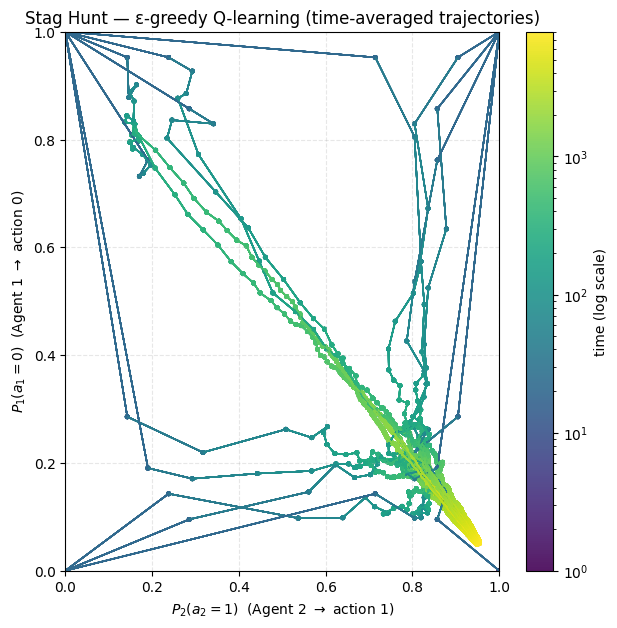
\includegraphics[width=\linewidth]{figures/task-2/learning/stag_hunt_egreedy.png}
        \caption*{(a) $\epsilon$-greedy Q-learning}
    \end{minipage}
    \hfill
    \begin{minipage}{0.32\textwidth}
        \centering
        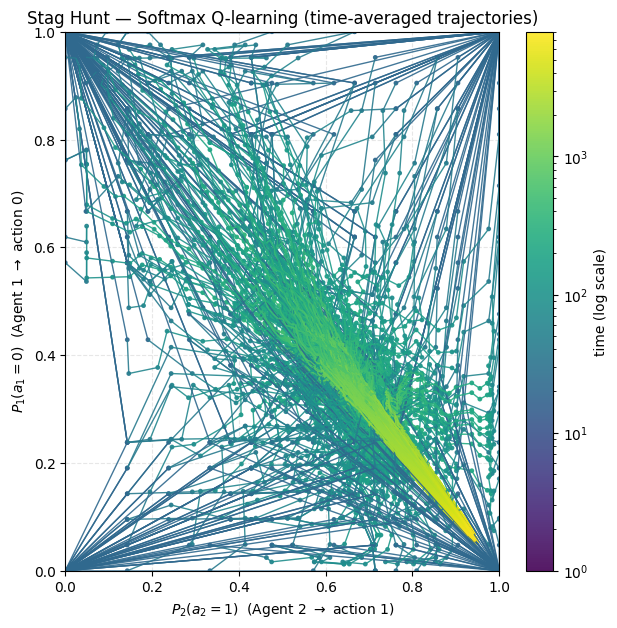
\includegraphics[width=\linewidth]{figures/task-2/learning/stag_hunt_boltz.png}
        \caption*{(b) Boltzmann Q-learning}
    \end{minipage}
    \hfill
    \begin{minipage}{0.32\textwidth}
        \centering
        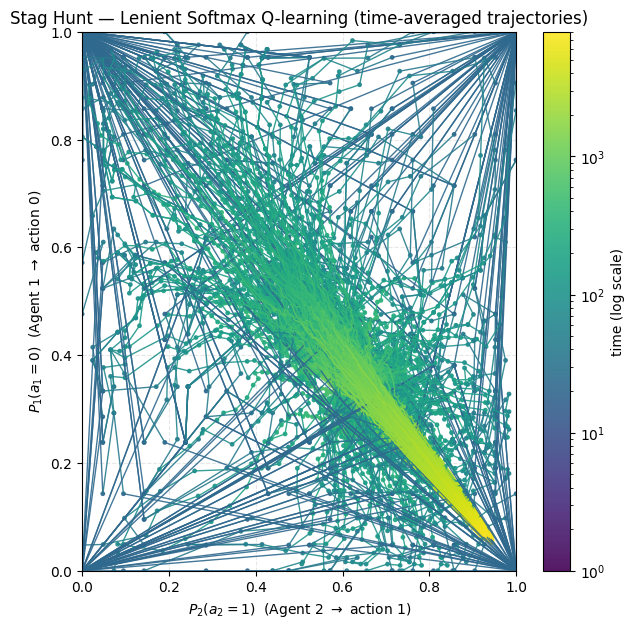
\includegraphics[width=\linewidth]{figures/task-2/learning/stag_hunt_lenient.png}
        \caption*{(c) Lenient Boltzmann Q-learning}
    \end{minipage}
    \caption{Empirical learning trajectories for the Stag Hunt game using (a) $\epsilon$-greedy Q-learning, (b) Boltzmann Q-learning, and (c) Lenient Boltzmann Q-learning.}
\end{figure}


\paragraph{Subsidy Game.}


Empirical learning trajectories for the Subsidy Game are shown below. For $\epsilon$-greedy Q-learning, agents rapidly converge to the dominant equilibrium $(S_1, S_1)$, as the incentives strongly favor this outcome. The trajectories are short, indicating fast convergence. Boltzmann Q-learning also converges to $(S_1, S_1)$, it does it so fast that the learning trajectories only show for when it learns the suboptimal policy. learing $(S_1, S_1)$ is just so quick. . Lenient Boltzmann Q-learning exhibits similar behavior, but the added leniency can result in slightly longer exploration before convergence, as agents are more tolerant of early mistakes.

\begin{figure}[h]
    \centering
    \begin{minipage}{0.32\textwidth}
        \centering
        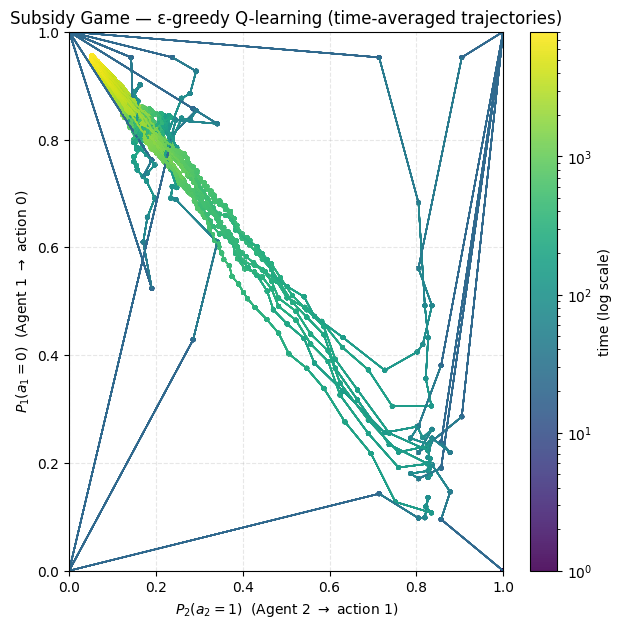
\includegraphics[width=\linewidth]{figures/task-2/learning/sg_egreedy.png}
        \caption*{(a) $\epsilon$-greedy Q-learning}
    \end{minipage}
    \hfill
    \begin{minipage}{0.32\textwidth}
        \centering
        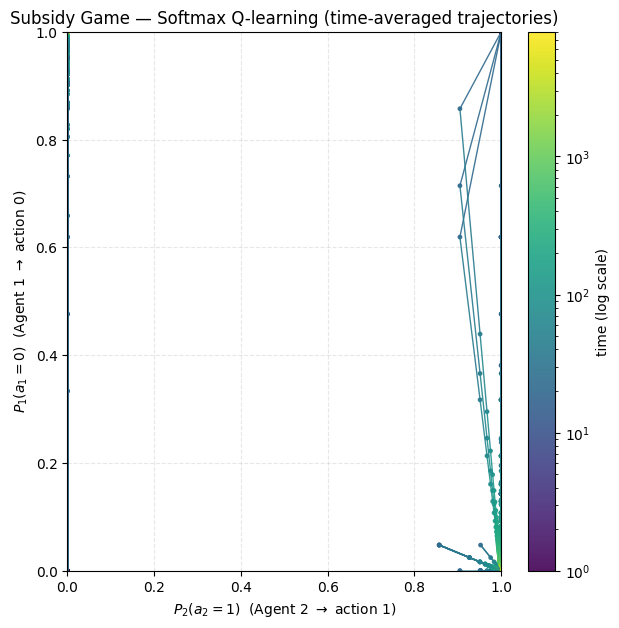
\includegraphics[width=\linewidth]{figures/task-2/learning/sg_boltz.png}
        \caption*{(b) Boltzmann Q-learning}
    \end{minipage}
    \hfill
    \begin{minipage}{0.32\textwidth}
        \centering
        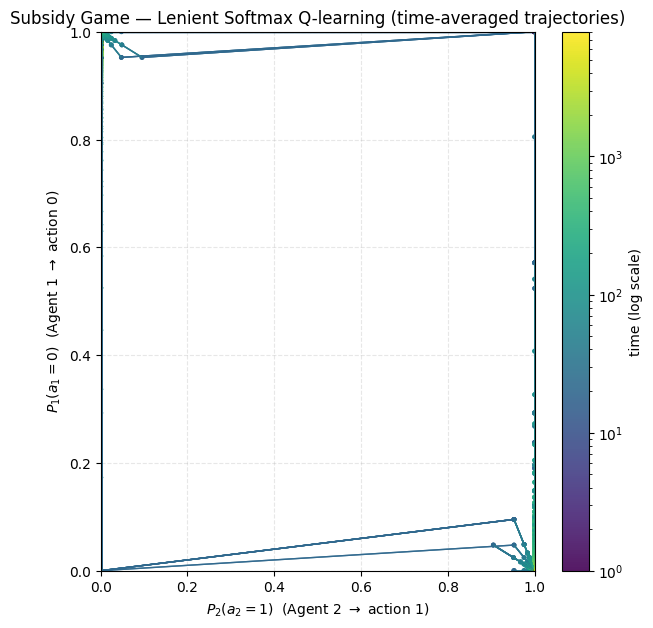
\includegraphics[width=\linewidth]{figures/task-2/learning/sg_lenient.png}
        \caption*{(c) Lenient Boltzmann Q-learning}
    \end{minipage}
    \caption{Empirical learning trajectories for the Subsidy Game using (a) $\epsilon$-greedy Q-learning, (b) Boltzmann Q-learning, and (c) Lenient Boltzmann Q-learning.}
\end{figure}


\paragraph{Matching Pennies.}
Empirical learning trajectories for Matching Pennies are shown below. The $\epsilon$-greedy Q-learning algorithm actually learns the mixed Nash equilibrium quite fast. Because of the decreasing exploration rate, the agent settles around the equilibrium. Boltzmann Q-learning also converges to the mixed strategy equilibrium, but the trajectories show more exploration around the equilibrium point, likely due to the softmax action selection. Lenient Boltzmann Q-learning exhibits similar behavior, with agents exploring more before settling into the mixed strategy equilibrium. The leniency allows for more exploration of suboptimal actions, but ultimately, agents converge to the Nash equilibrium.

\begin{figure}[h]
    \centering
    \begin{minipage}{0.32\textwidth}
        \centering
        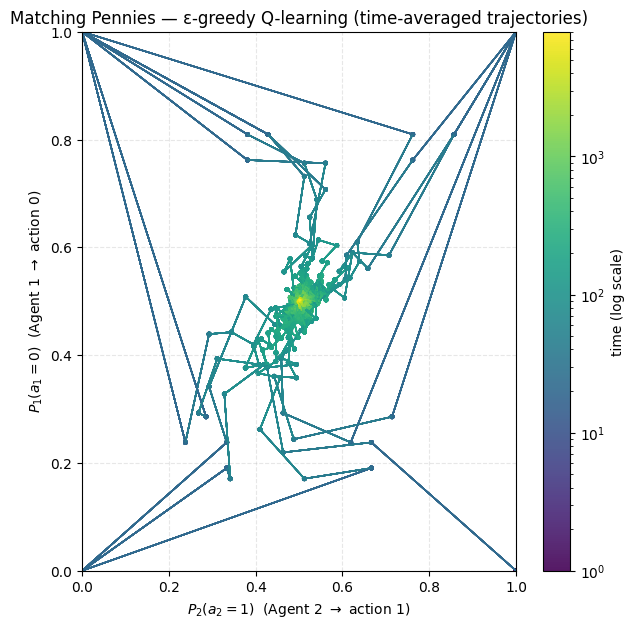
\includegraphics[width=\linewidth]{figures/task-2/learning/mp_egreedy.png}
        \caption*{(a) $\epsilon$-greedy Q-learning}
    \end{minipage}
    \hfill
    \begin{minipage}{0.32\textwidth}
        \centering
        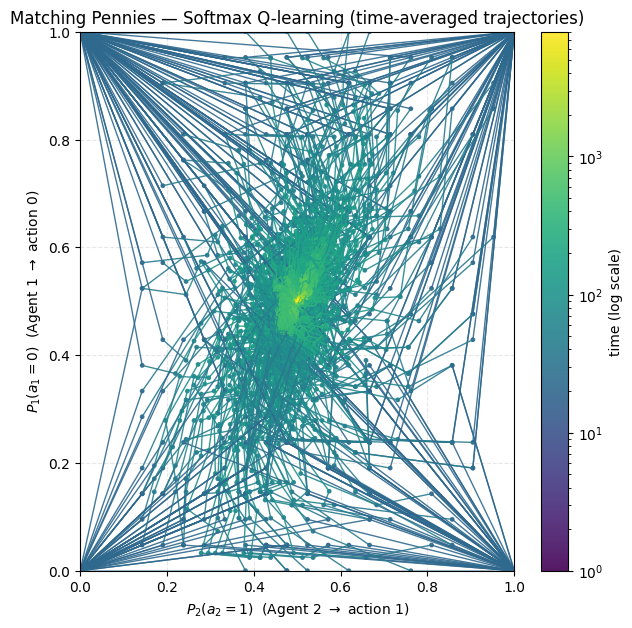
\includegraphics[width=\linewidth]{figures/task-2/learning/mp_boltz.png}
        \caption*{(b) Boltzmann Q-learning}
    \end{minipage}
    \hfill
    \begin{minipage}{0.32\textwidth}
        \centering
        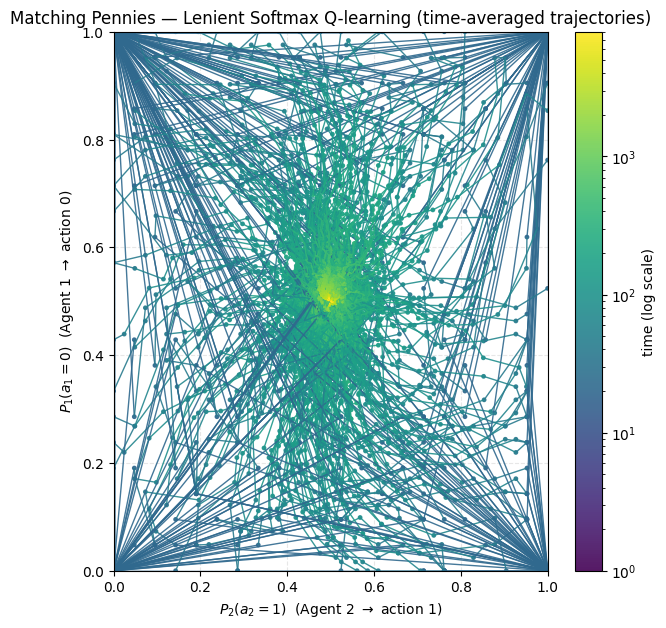
\includegraphics[width=\linewidth]{figures/task-2/learning/mp_lenient.png}
        \caption*{(c) Lenient Boltzmann Q-learning}
    \end{minipage}
    \caption{Empirical learning trajectories for Matching Pennies using (a) $\epsilon$-greedy Q-learning, (b) Boltzmann Q-learning, and (c) Lenient Boltzmann Q-learning.}
\end{figure}


\paragraph{Prisoner’s Dilemma.}
Empirical learning trajectories for the Prisoner’s Dilemma are shown below. The $\epsilon$-greedy Q-learning algorithm quickly converges to the dominant strategy $(D,D)$, as defection strictly dominates cooperation. The trajectories are short, indicating fast convergence. Boltzmann Q-learning also converges to $(D,D)$, with trajectories showing some exploration of cooperative strategies before settling into defection. Lenient Boltzmann Q-learning exhibits similar behavior, but the added leniency allows for slightly longer exploration of cooperative strategies before ultimately converging to the Nash equilibrium of mutual defection.             


\begin{figure}[h]
    \centering
    \begin{minipage}{0.32\textwidth}
        \centering
        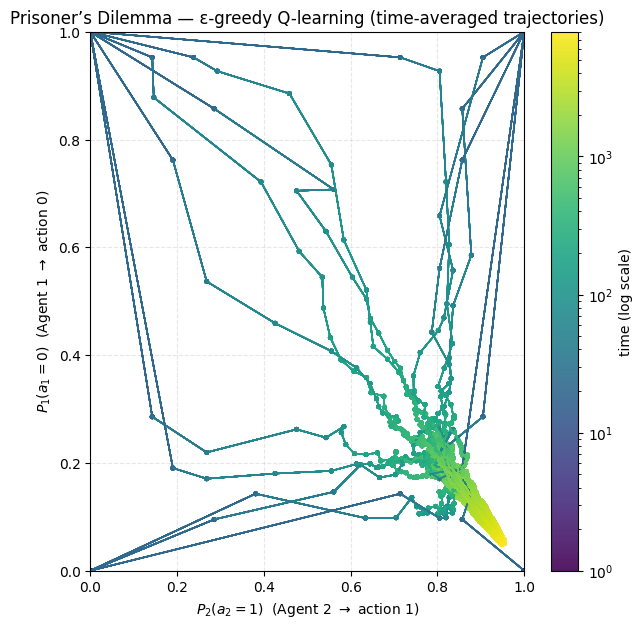
\includegraphics[width=\linewidth]{figures/task-2/learning/pd_egreedy.png}
        \caption*{(a) $\epsilon$-greedy Q-learning}
    \end{minipage}
    \hfill
    \begin{minipage}{0.32\textwidth}
        \centering
        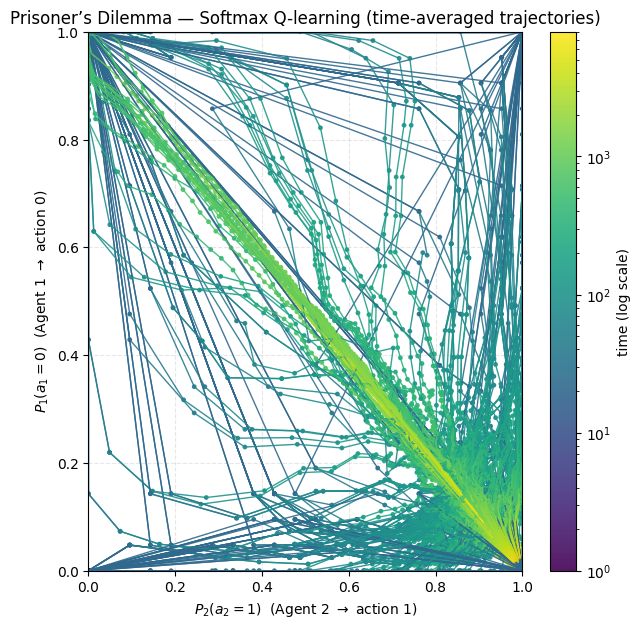
\includegraphics[width=\linewidth]{figures/task-2/learning/pd_boltz.png}
        \caption*{(b) Boltzmann Q-learning}
    \end{minipage}
    \hfill
    \begin{minipage}{0.32\textwidth}
        \centering
        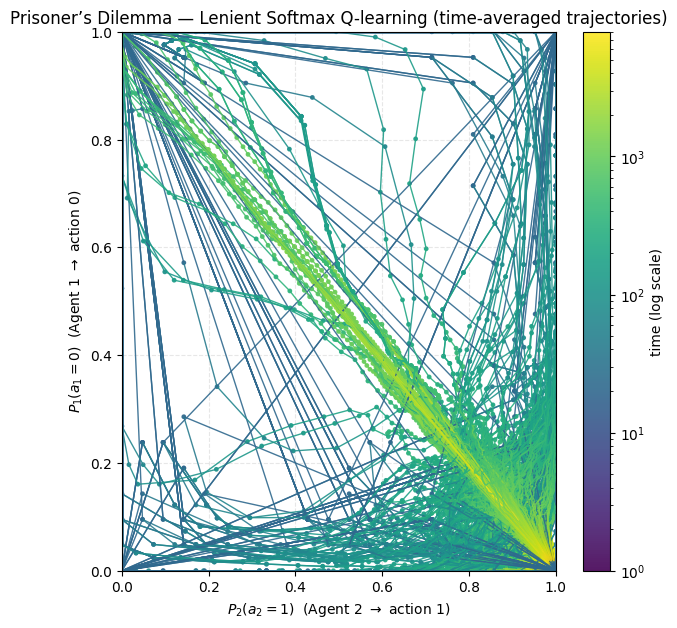
\includegraphics[width=\linewidth]{figures/task-2/learning/pd_lenient.png}
        \caption*{(c) Lenient Boltzmann Q-learning}
    \end{minipage}
    \caption{Empirical learning trajectories for the Prisoner's Dilemma using (a) $\epsilon$-greedy Q-learning, (b) Boltzmann Q-learning, and (c) Lenient Boltzmann Q-learning.}
\end{figure}



\subsection{Analitical analysis of the learning dynamics using replicator equations}
The learning dynamics of the algorithms are analyzed using replicator equations, which model how the proportion of strategies in a population change over time based on their relative payoffs. The replicator equations are visualized as vector fields over the strategy simplex, with arrows indicating the direction and magnitude of change in strategy proportions. The replicator dynamics of each game are plotted for Boltzmann Q-learning and Lenient Boltzmann Q-learning. The derivation of the equations and the implementation are in an appended notebook for clarity and reproducibility.

\begin{figure}
    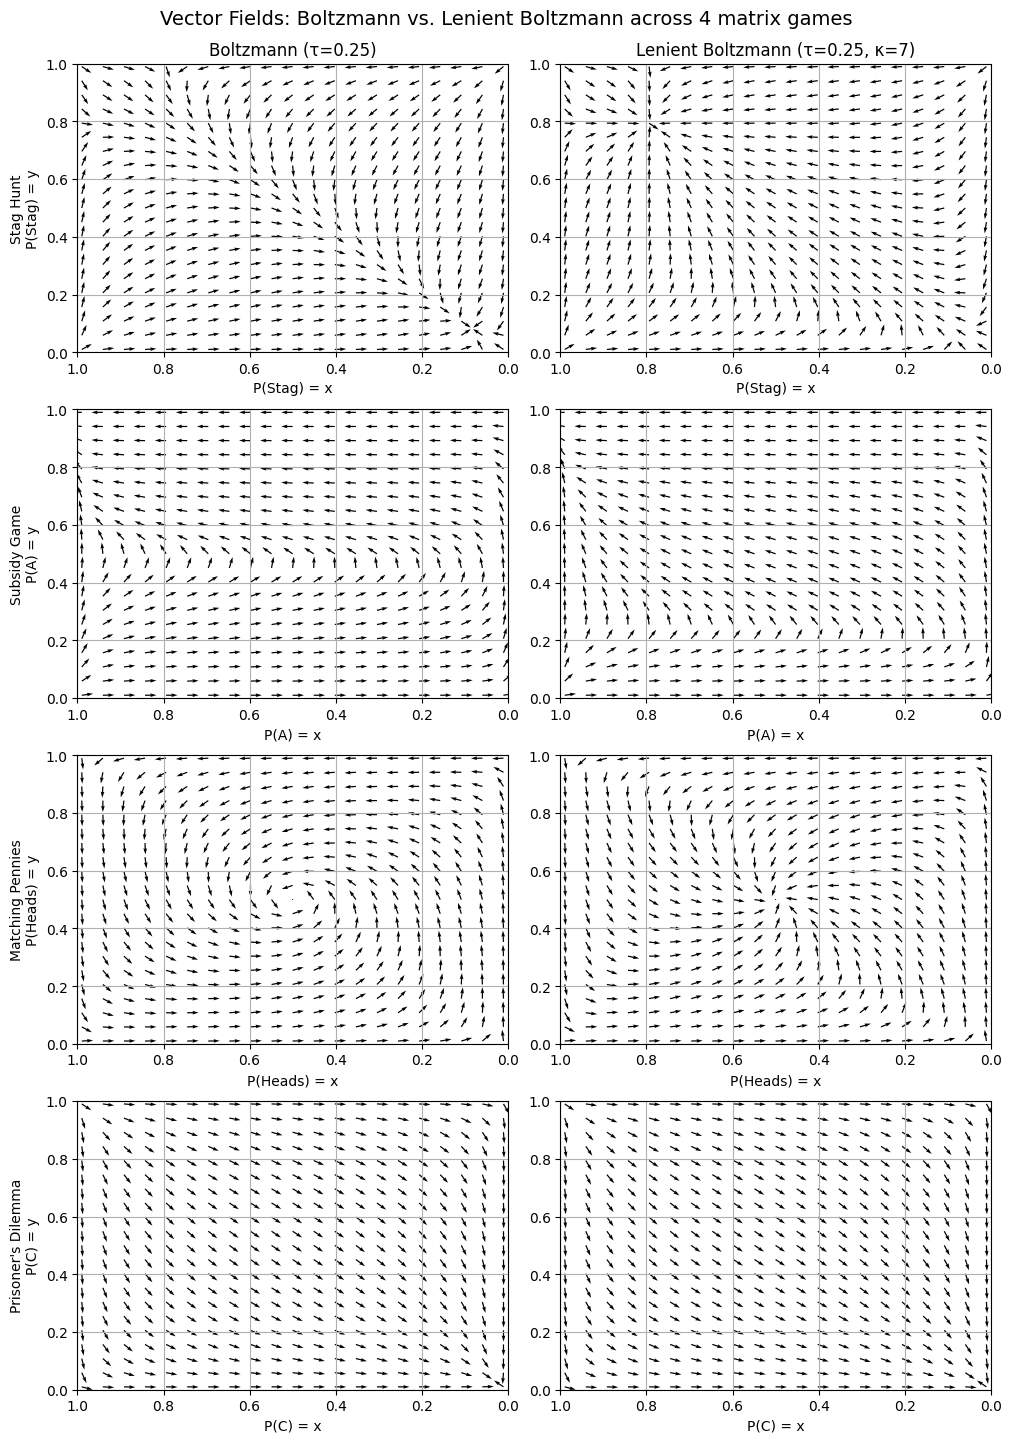
\includegraphics[width=\linewidth]{figures/task-2/replicator_dynamics.png}
\end{figure}

The learning behavior observed in the empirical trajectories match well with the predictions made by the replicator equations, confirming the validity of the analytical approach. The only inconsistency is that the replicator dynamics predict that Lenient Boltzmann Q-learning should be able to learn to cooperate in the Stag Hunt, while the empirical results show that it fails to do so. This discrepancy could be due to the specific parameters used in the learning algorithms, such as the learning rate, exploration rate, and leniency factor. Further tuning of these parameters might help align the empirical results with the theoretical predictions.

